\section{Auswertung}
\label{sec:Auswertung}
\subsection{Abbildungsgleichung}
Die Messwerte die zur Verifizierung der Gleichung \eqref{eqn:linsengleichung} aufgenommen wurden, sind in Tabelle \ref{tab:abbildung} zu finden.
\begin{table}
    \centering
    \begin{tabular}{ccc}
    \toprule
    $b \,/\, \si{\centi\meter}$ & $g \,/\, \si{\centi\meter}$ & $B \,/\, \si{\centi\meter}$ \\
    \midrule
    34.8 & 25 &  2.9 \\
    27.6 & 30 &  2.6 \\
    24.4 & 35 &  2.0 \\
    22.5 & 40 &  1.6 \\
    21.0 & 45 &  1.4 \\
    20.0 & 50 &  1.1 \\
    \bottomrule
    \end{tabular}
    \caption{Die Messwerte für den Abstand von Linse zu Schirm $b$, von Linse zu Gegenstand $g$, und der Abbildungsgröße auf dem Schirm $B$.}
\label{tab:abbildung}
\end{table}

Aus diesen Werten wurde nun mithilfe der Gleichung \eqref{eqn:linsengleichung} die Brennweite der Linse berechnet.
Die berechneten Brennweiten sind in Tabelle \ref{tab:brennweiten_bessel} zu finden

\begin{table}
    \centering
    \begin{tabular}{c}
    \toprule
    $f \,/\, \si{\centi\meter}$  \\
    \midrule
    14.54     \\
    14.37     \\
    14.37    \\
    14.40     \\
    14.31    \\
    14.28   \\
    \bottomrule
    \end{tabular}
    \caption{Die aus Gleichung \eqref{eqn:linsengleichung} berechneten Brennweiten.}
    \label{tab:brennweiten_bessel}
\end{table}

Der Mittelwert der berechneten Brennweiten beträgt 
\begin{align*}
 \bar{f} & =  \SI{14.384(37)}{\centi\meter}\\
\end{align*}
und weicht damit um $\Delta \bar{f} = \SI{0.62(4)}{\centi\meter}$ von der tatsächlichen Brennweite von $\SI{15}{\centi\meter}$ ab.
Aus den Messwerte in Tabelle \ref{tab:abbildung} wurde zudem ein Plot erstellt, der in Abbildung \ref{fig:brennweite} zu sehen ist.
Der Plot wurde mit dem python Paket matplotlib \cite{matplotlib} erstellt.
Um die Schnittpunkte und den Schwerpunkt der Schnittpunkte besser erkennen zu können wurde der Bereich um den Schwerpunkt vergrößert.
Die vergrößerte Abbildung ist in Grafik \ref{fig:zoom} zu sehen.
\begin{figure} 
    \centering
    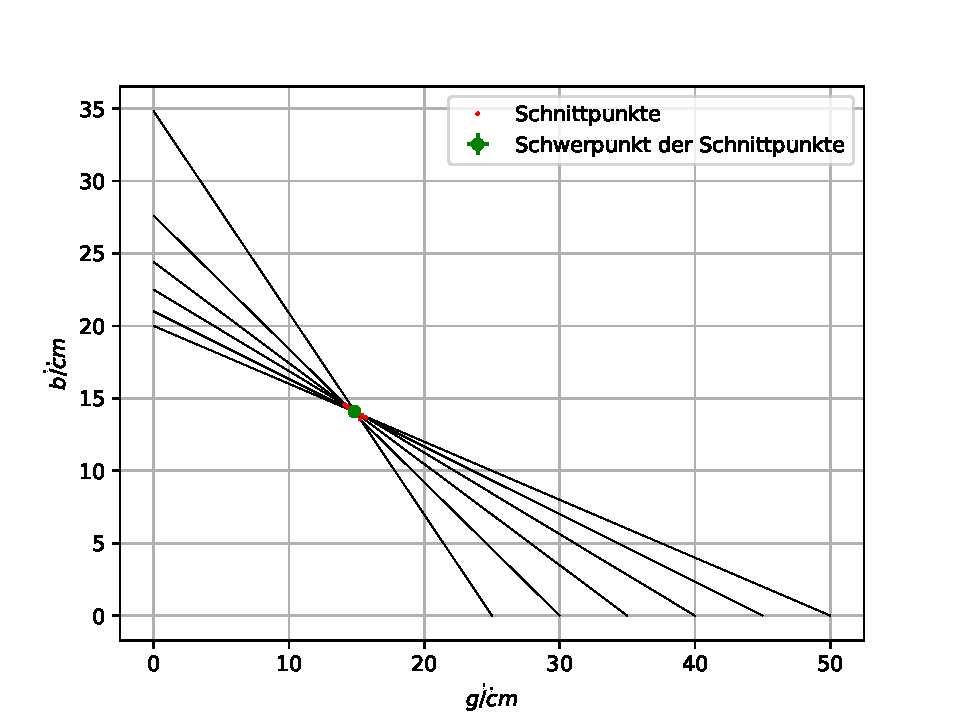
\includegraphics[width=\textwidth]{content/data/brennweite.pdf}
    \caption{Die aufgenommenen Werte Paare, verbunden mit einer Gerade um die Messgenauigkeit und die Brennweite der Linse zu erkennen.}
    \label{fig:brennweite}
\end{figure}
\begin{figure}
    \centering
    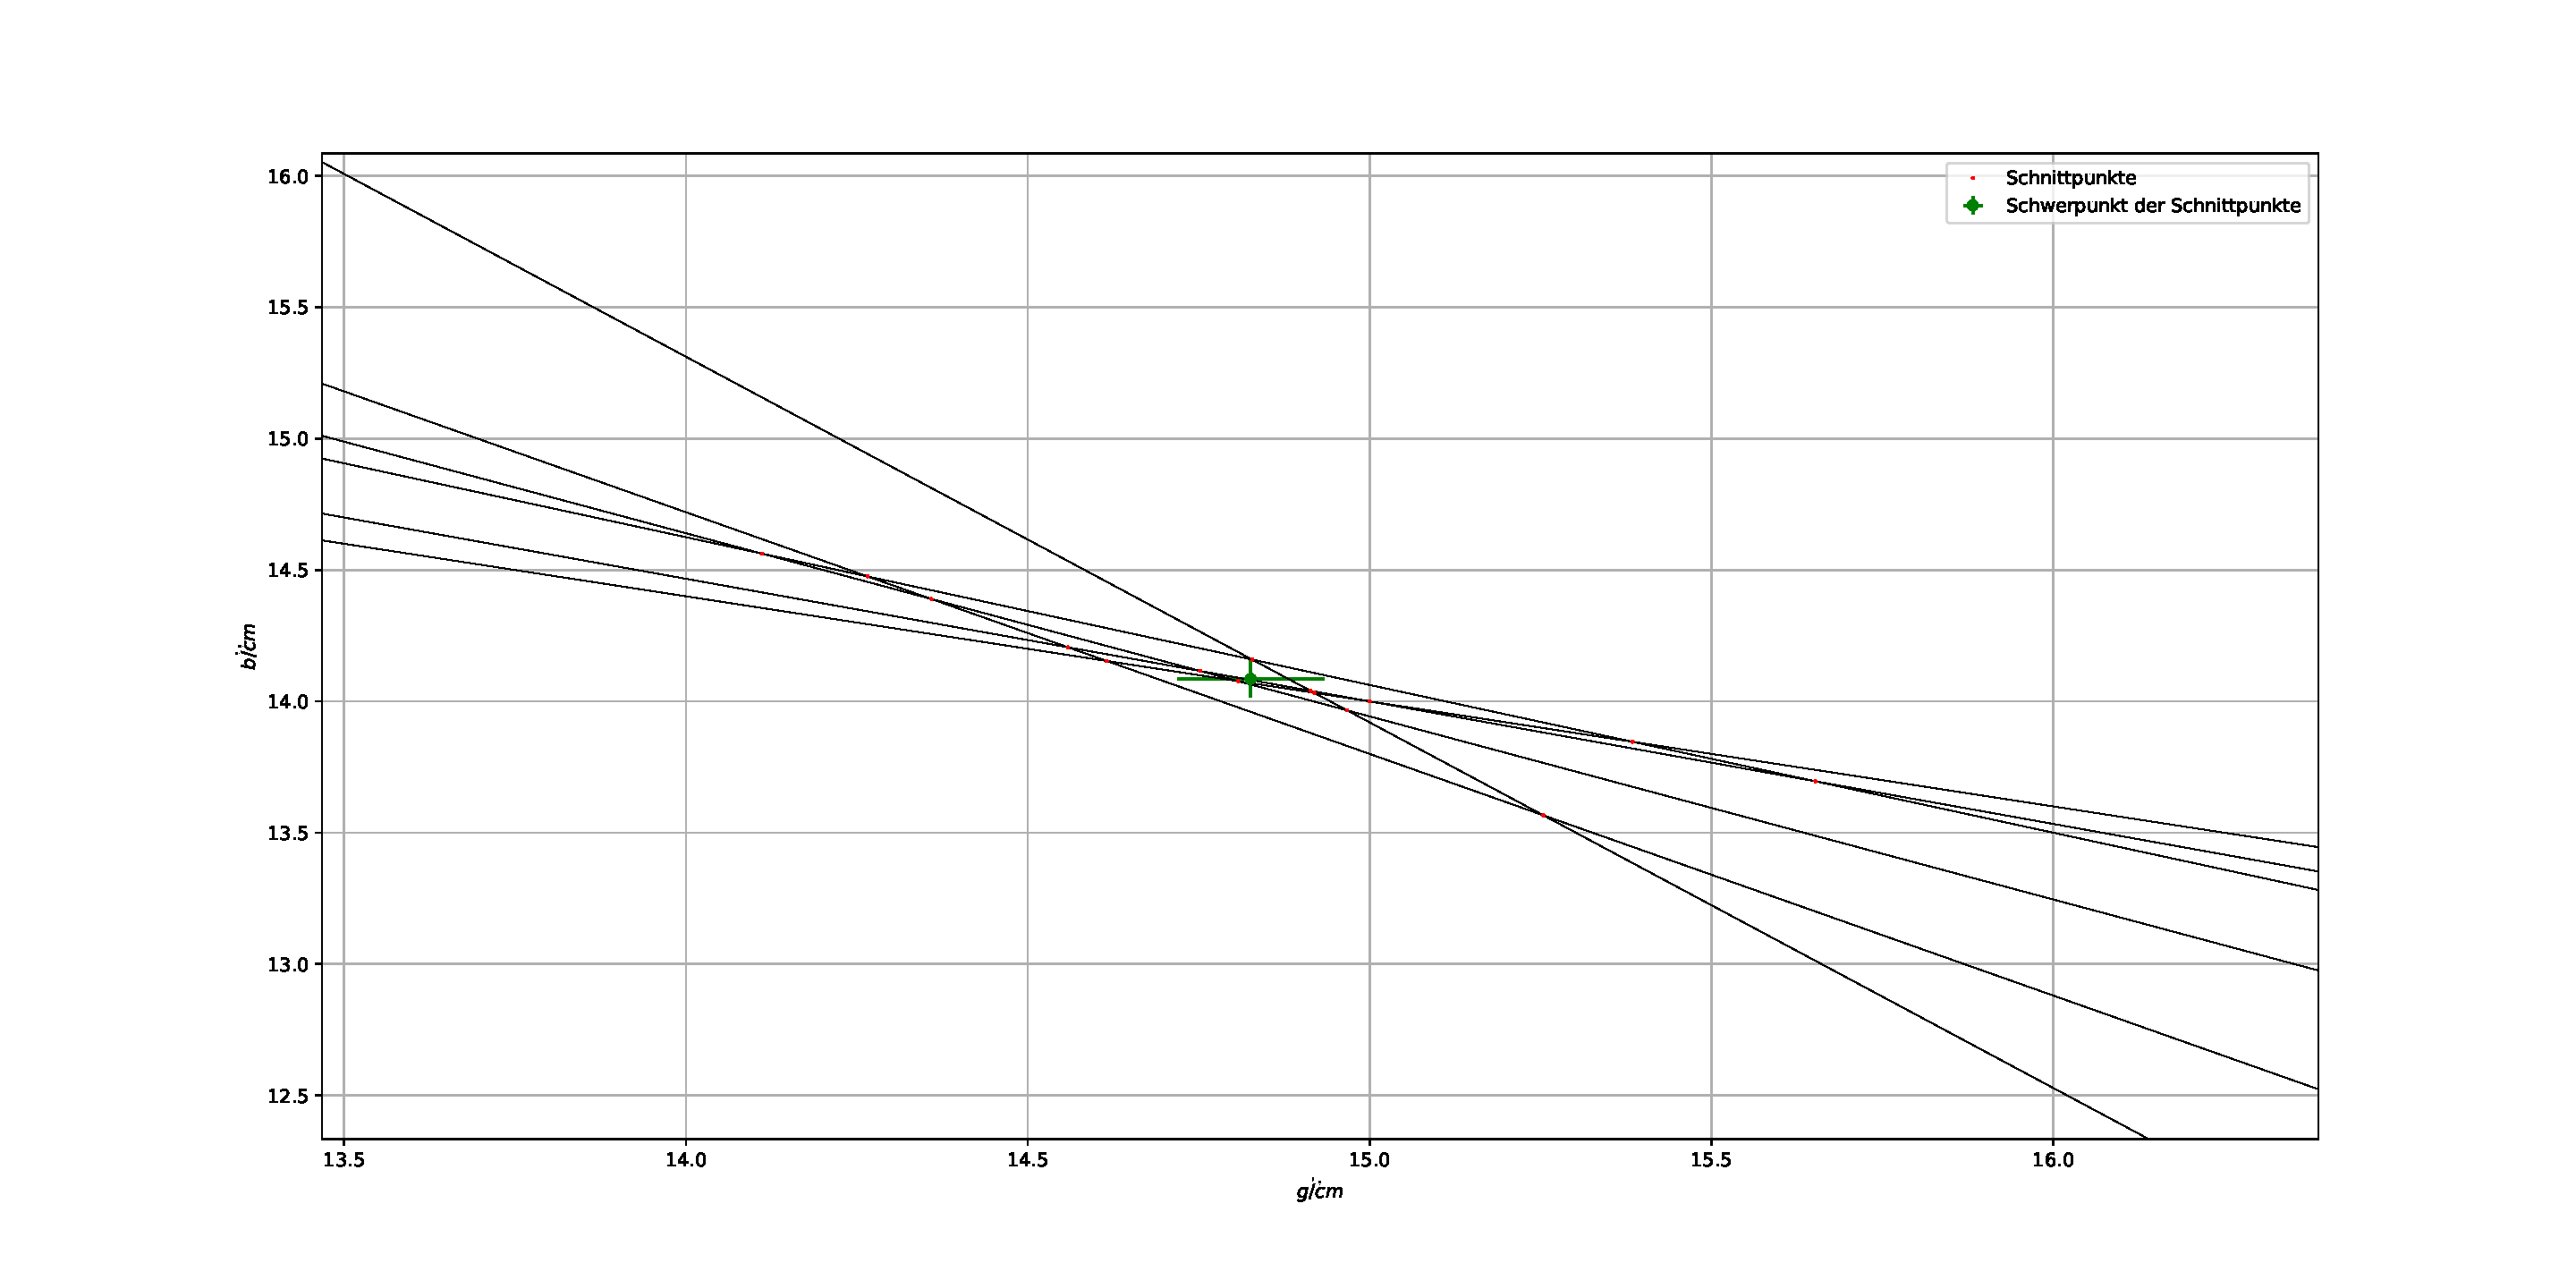
\includegraphics[width=\textwidth]{content/data/zoom_schnittpunkt.pdf}
    \caption{Die Abbildung \ref{fig:brennweite} um den Schwerpunkt der Schnittpunkte herum vergößert.}
    \label{fig:zoom}
\end{figure}
Dafür wurden durch jedes Werte Paar eine Gerade gezogen.
Die Schnittpunkte der Geraden wurden rot markiert.
Aus den Schniitpunkten wurde dann der Schwerpunkt dieser bestimmt und grün markiert.
Die Schnittpunkte der Geraden wurden dabei durch gleichsetzten der jeweiligen Geradengleichungen berechnet.
Der Schwerpunkt $S$ aller Schnittpunkte wurde jeweils getrennt für die $x$- und $y$-Koordinate berechnet.
Dafür wurde der Mittelwert aus alles Schnittpunkten berechnet.
Der Mittelwert der Schnittpunkte liegt bei 
\begin{align*}
    S_\text{x} & =  \SI{14.83(11)}{\centi\meter}\\
    S_\text{y} & =  \SI{14.09(7)}{\centi\meter}. \\
\end{align*}
Wie zu erkennen ist weicht auch dieser von der eigentlichen Brennweite ab.
Die Abweichung betragen dabei 
\begin{align*}
   \Delta S_\text{x} & =  \SI{0.17(11)}{\centi\meter} \\
    \Delta S_\text{y} & =  \SI{0.91(7)}{\centi\meter}. \\
\end{align*}
Mit der Gleichung \eqref{eqn:abbildungsgesetz} wurde zudem der Abbildungsmaßstab $V$ berechnet.
Einmal durch die Messwerte der Bildgröße $B$ und der Gegenstandsgröße $G$, dieser Abbildungsmaßstab soll $V_1$ heißen, und einmal zum Vergleich mit den Abständen $g$ und $b$, dieser heißt $V_2$.
Aus den berechneten Abbildungsgrößen wurde zudem der Mittelwert berechnet um das weitere rechnen übersichtlicher zu gestalten.
Die berechneten Mittelwerte sind 
\begin{align*}
    \bar{V_1} & =  \SI{0.64(10)}{}\\
    \bar{V_2} & =  \SI{0.74(15)}{}.
\end{align*}
Damit weichen sie um $\Delta \bar{V} = \SI{0.10(18)}{}$ voneinander ab.

\subsection{Bestimmung einer unbekannten Brennweite durch Bessel}
Die Messwerte die durch die Bessel'schen Methode aufgenommen wurden sind in Tabelle \ref{tab:bessel_weiß} zu sehen.
Zudem wurden die selbe Methode für rotes und blaues Licht durchgeführt, die Messwerte dieser Messungen sind in Tabelle \ref{tab:rot} für rotes Licht und in Tabelle \ref{tab:blau} für blaues Licht, zu sehen.
\begin{table}
    \centering
    \begin{tabular}{ccc}
    \toprule
    $e\,/\,\si{\centi\meter}$ & $b\,/\, \si{\centi\meter}$ & $ g\,/\, \si{\centi\meter} $ \\
    75 & 55.5 & 19.5    \\
    75 & 19.3 & 55.7    \\
    80 & 19.1 & 60.9    \\
    80 & 61.4 & 18.6    \\
    85 & 18.7 & 66.3    \\
    85 & 67.0 & 18.0    \\
    90 & 18.5 & 71.5    \\
    90 & 72.0 & 18.0    \\
    100 & 17.9 & 82.1   \\
    100 & 82.7 & 17.3   \\
    110 & 17.5 & 92.5   \\
    110 & 93.3 & 16.7   \\
    \bottomrule
    \end{tabular}
    \caption{Die bei der Bessel'schen Methode aufgenommenen Abstände von Schirm zu Gegenstand $e$, von Linse zu Schirm $b$ und von Gegenstand zu Linse $g$.}
    \label{tab:bessel_weiß}
\end{table}

\begin{table}
    \centering
    \begin{tabular}{cc}
    \toprule
    $e\,/\,\si{\centi\meter}$ & $b\,/\, \si{\centi\meter}$\\
    64 & 22.7 \\
    64 & 42.0 \\
    70 & 21.1 \\
    70 & 49.4 \\
    80 & 19.4 \\
    80 & 61.1 \\
    \bottomrule
    \end{tabular}
    \caption{Die bei der Bessel'schen Methode aufgenommenen Abstände von Schirm zu Gegenstand $e$, von Linse zu Schirm $b$, für rotes Licht}
    \label{tab:rot}
\end{table}

\begin{table}
    \centering
    \begin{tabular}{cc}
    \toprule
    $e\,/\,\si{\centi\meter}$ & $b\,/\, \si{\centi\meter}$\\
    64 &  22.4 \\
    64 &  42.2 \\
    70 &  20.6 \\
    70 &  50.1 \\
    80 &  19.2 \\
    80 &  61.4 \\
    \bottomrule
    \end{tabular}
    \caption{Die bei der Bessel'schen Methode aufgenommenen Abstände von Schirm zu Gegenstand $e$, von Linse zu Schirm $b$, für blaues Licht}
    \label{tab:blau}
\end{table}

Aus diesen Werten wurden die Brennweiten durch Gleichung \eqref{eqn:bessel} berechnet.
Die berechneten Brennweiten für weißes Licht sind in der Tabelle \ref{tab:brennweiten_weis} zu finden.
Die für blaues und rotes Licht sind in Tabelle \ref{tab:blau_rot}
\begin{table}
    \centering
    \begin{tabular}{c}
    \toprule
    $f_\text{weiß} \,/\, \si{\centi\meter}$ \\
    \midrule
    14.43\\
    14.33\\
    14.53\\
    14.27\\
    14.58\\
    14.18\\
    14.69\\
    14.4\\
    14.69\\
    14.30\\
    14.71\\
    14.16\\
    \bottomrule
    \end{tabular}
    \caption{Die aus Gleichung \eqref{eqn:bessel} berechneten Brennweiten für weißes Licht.}
    \label{tab:brennweiten_weis}
\end{table}

\begin{table}
    \centering
    \begin{tabular}{cc}
    \toprule
    $f_\text{rot} \,/\, \si{\centi\meter}$ & $f_\text{blau} \,/\, \si{\centi\meter}$ \\
    \midrule
    14.64 & 14.56 \\
    14.43 & 14.37\\
    14.73 & 14.53\\
    14.53 & 14.24\\
    14.69 & 14.59\\
    14.43 & 14.27\\
    \bottomrule
    \end{tabular}
    \caption{Die aus Gleichung \eqref{eqn:bessel} berechneten Brennweiten für rotes und blaues Licht.}
    \label{tab:blau_rot}
\end{table}

Aus den berechneten Brennweiten wurden die Mittelwerte der Brennweiten berechnet diese betragen
\begin{align*}
    \bar{f_\text{weiß}} & =  \SI{14.44(6)}{\centi\meter} \\
    \bar{f_\text{rot}}  & =  \SI{14.58(5)}{\centi\meter} \\
    \bar{f_\text{blau}} & =   \SI{14.43(6)}{\centi\meter} \\
\end{align*}


\subsection{Methode von Abbe}

Die Messwerte die bei der Abbe'schen Methode aufgenommen wurden sind in Tablle \ref{tab:abbe} zu finden.
\begin{table}
    \centering
    \begin{tabular}{ccc}
        \toprule
        $g \,/\, \si{\centi\meter} $&$ b\,/\, \si{\centi\meter} $&$ B \,/\, \si{\centi\meter} $\\
        14.1 & 65.9 & 12.0   \\
        17.0 & 38.7 & 5.8 \\
        20.0 & 30.4 & 3.9 \\
        23.0 & 25.3 & 2.8 \\
        26.0 & 23.3 & 2.2 \\
        29.0 & 21.7 & 1.9 \\
    \end{tabular}
    \caption{Die Abstände von Gegenstand zur ersten Hauptebene des Linsenpaares $g$, von zweiter Hauptebene zum Schirm $b$ und die Abbildungsgröße $G$.}
    \label{tab:abbe}
\end{table}

Diese Messwerte wurden zunächst grafisch aufgetragen.
Dafür wurde aus den Messwerte der Abbildungsgröße und der Gegenstandsgröße nach \eqref{eqn:abbildungsgesetz} der Abbildungsmaßstab $V$ berechnet.
Gegen diesen wurden nun $g$ und $b$ aufgetragen. 
Die Plots sind in Abbildung \ref{fig:abbe} zu sehen.

\begin{figure}
    \centering
    \begin{subfigure}{0.48\textwidth}
        \centering
        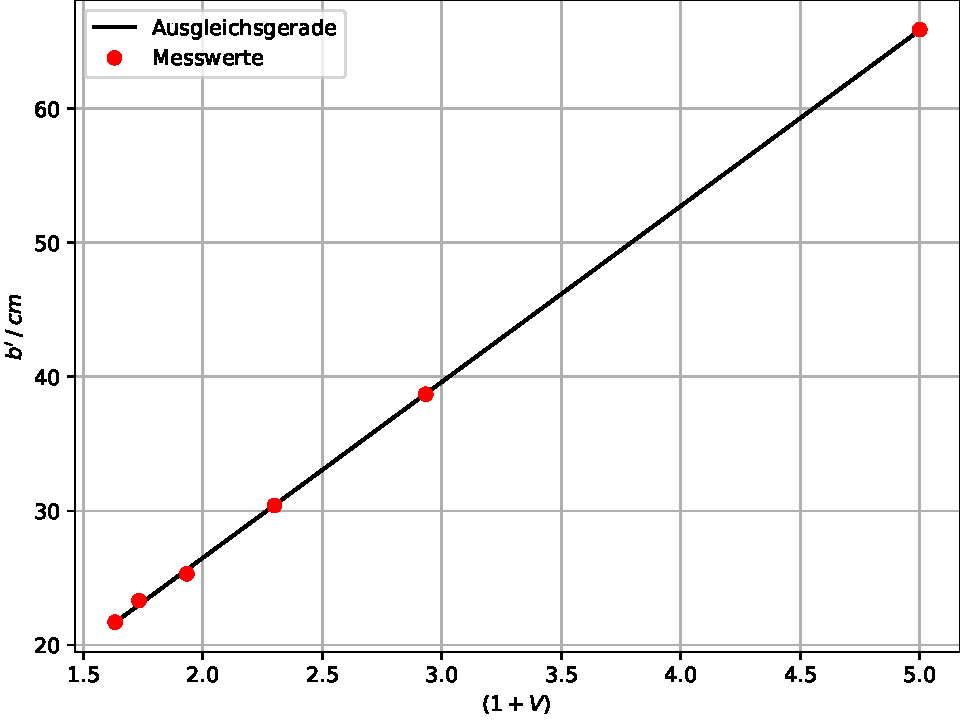
\includegraphics[width=\textwidth]{content/data/plot_abbe_b.pdf}
        %\caption{Der Plot zu $b$}
        %\label{fig:plotb}
    \end{subfigure}
    \begin{subfigure}{0.48\textwidth}
        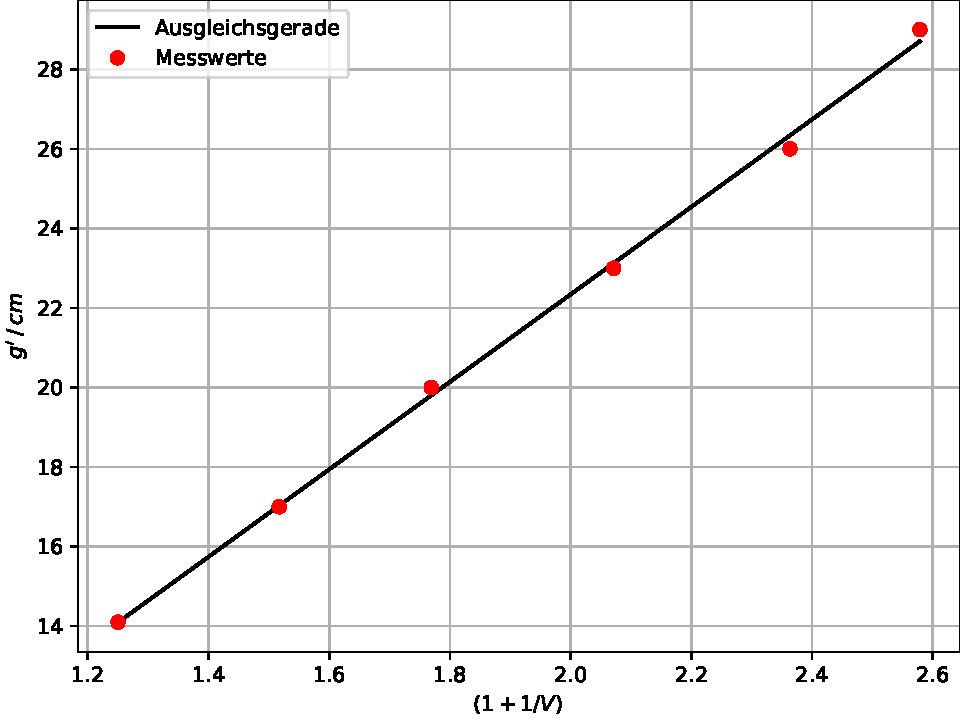
\includegraphics[width=\textwidth]{content/data/plot_abbe_g.pdf}
        %\caption{Der Plot zu $a$}
    \end{subfigure}
    \caption{Die beiden Plots für die Messwerte die beide Methode nach Abbe aufgenommen wurde.}
    \label{fig:abbe}
\end{figure}

Die Ausgleichsgeraden wurden dabei mit dem Python Paket scipy \cite{scipy} erstellt.
Die Ausgleichsgeraden wurden mit der Gleichung 
\begin{align}
    g' &= f \cdot \left( 1+\frac{1}{V} \right) + h \label{eq:abbe_g} \\
    b' &= f \cdot \left( 1+V \right) + h' \, .
    \label{eq:abbe_b}
\end{align}
erstellt.
Das $h$ entspricht dabei dem Abstand von Hauptebene zu $g$ oder $b$.
Aus diesem Grund entsprechen $g$ und $b$ auch nicht genau $g'$ und $b'$.
Die Parameter der Ausgleichsgeraden werden auf 
\begin{align*}
    f_{g'} = \SI{11.00(22)}{\centi\meter}, & \,\,h = \SI{0.3(4)}{\centi\meter}\\
    f_{b'} = \SI{13.12(8)}{\centi\meter}, & \,\, h = \SI{0.24(22)}{\centi\meter}
\end{align*}
bestimmt.
